% \section{数学工具}
% \subsection{拉普拉斯分布}
% % 合成图像数据集往往假设低分辨率图像由高分辨率图像经高斯模糊和双三次下采样得到,使用公式表示即为:
% % \begin{equation}
% %     \mathbi{I}^{LR}=(\vb*{k}_g\otimes \mathbi{I}^{HR})\downarrow_s
% % \end{equation}
% 拉普拉斯分布是以法国数学家Pierre-Simon命名的一种连续概率分布,又称双指数分布。拉普拉斯分布的概率密度函数为
% \begin{equation}
%     f(x;\mu, b)=\frac{1}{2b}\exp(-\frac{|x-\mu|}{b})
% \end{equation}
% 其中,$\mu$为位置参数,表示其对称轴位置;$b$为尺度参数,表示其开口尺度。其概率密度函数与累计分布函数如图\ref{fig:laplace-a}\ref{fig:laplace-b}所示。在本文所基于的模型USR-DU中,作者经过实验发现真实的低分辨率图像与双三次下采样图像之间的差异呈拉普拉斯分布,如图\ref{fig:laplace-c}所示。
% \begin{figure}[h]
%     \subcaptionbox{\label{fig:laplace-a}}{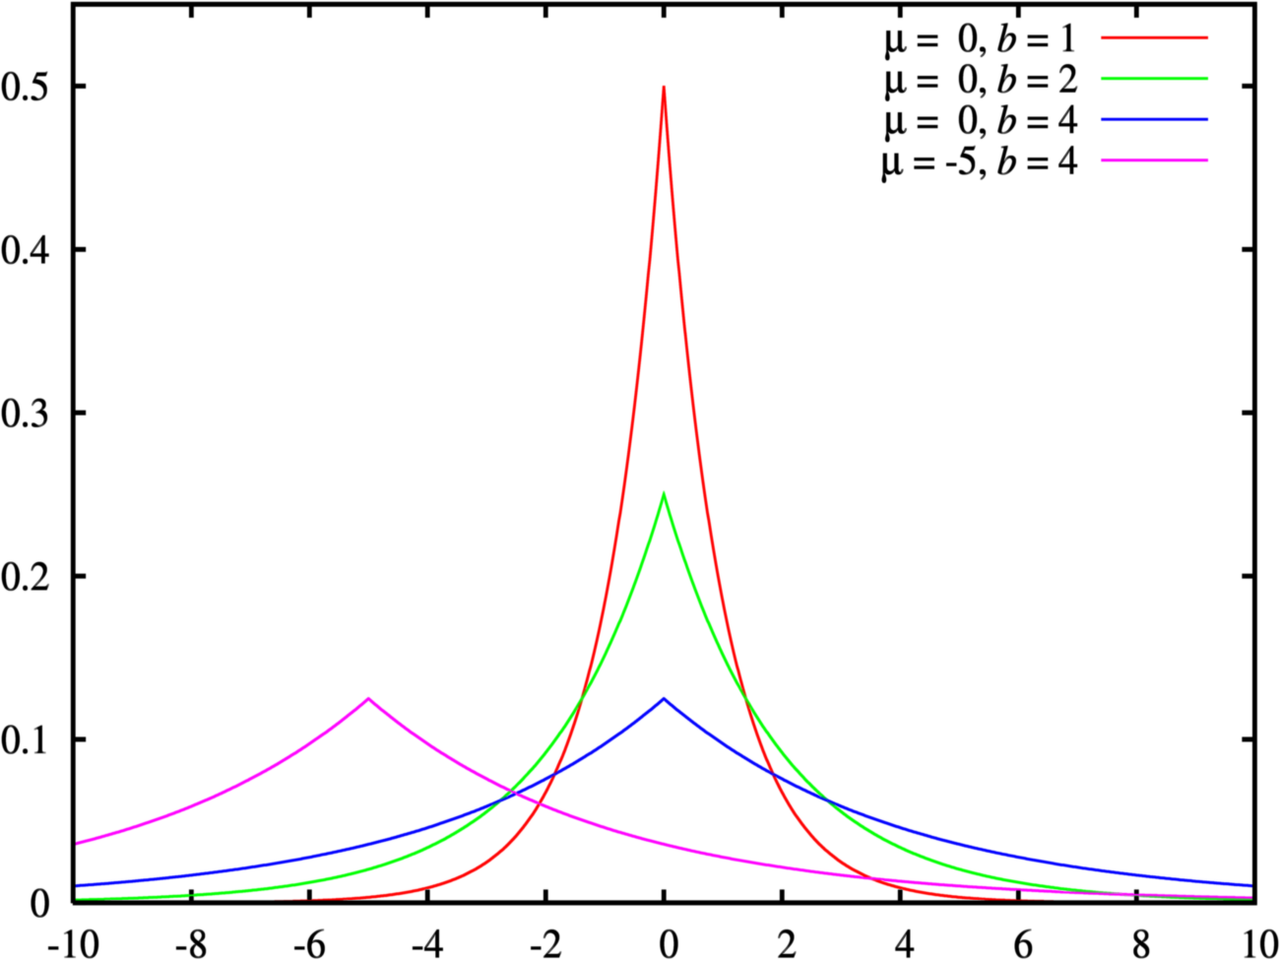
\includegraphics[width=.3\linewidth]{imgs/laplace_wiki_1.png}}\hfill
%     \subcaptionbox{\label{fig:laplace-b}}{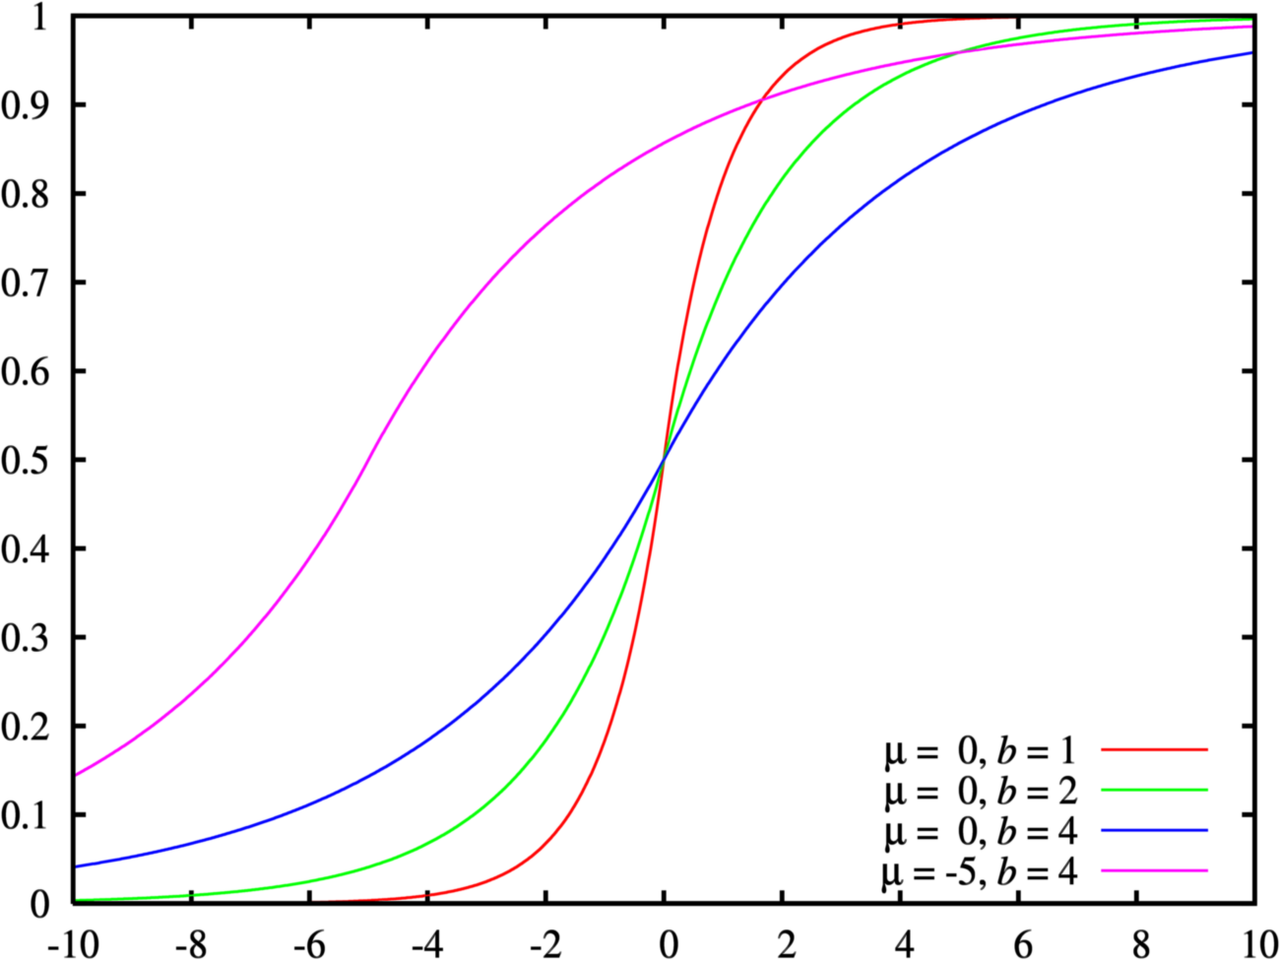
\includegraphics[width=.3\linewidth]{imgs/laplace_wiki_2.png}}\hfill
%     \subcaptionbox{\label{fig:laplace-c}}{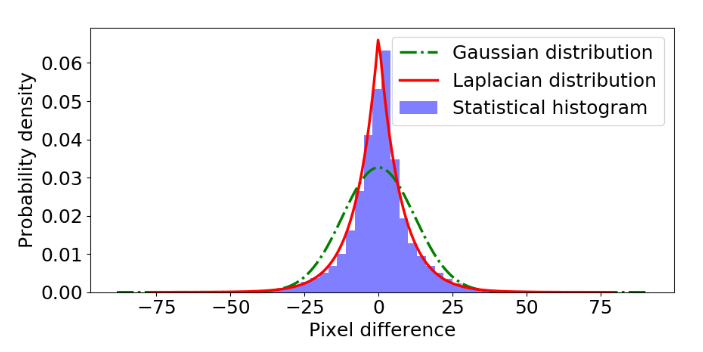
\includegraphics[width=.4\linewidth]{imgs/laplace_usr-du.png}}
%     \caption{拉普拉斯分布:其中,图(a)为概率密度函数,图(b)为累计分布函数,图(c)为USR-DU论文中作者对真实低分辨率图像与双三次下采样图像间差异分布进行实验的结果,作者发现实际的分布近似于拉普拉斯分布而不近似于高斯分布}	
%     \label{fig:laplace}
% \end{figure}

% \subsection{KL散度}
% KL散度(Kullback-Leibler divergence)又称相对熵,描述了$P$,$Q$两个分布之间的差异,其中$P$为真实分布,$Q$为估计分布。对于连续随机变量,KL散度可定义为
% \begin{equation}
%     D_{\text{KL}}(P\|Q)=\int^\infty_{-\infty}p(x)\ln\frac{p(x)}{q(x)}\,\text{d}x
% \end{equation}

% 在USR-DU中,DSN输出低分辨率图像$\vb*{y}_g$及其不确定性$\bm{\theta}$,其实质为输出了估计的低分辨率图像的分布。故为了优化网络,使其估计出正确的分布,可使用KL散度来构造损失函数
% \begin{equation}
%     \begin{aligned}
%         \mathcal{L}_{kl}&=\mathbb{E}_{\vb*{y}_g}\{D_{\text{KL}}[L(\vb*{y}_g,\bm{\theta})\|L(\vb*{y}_b,\mathbi{I})]\}  \\
%         &=\mathbb{E}_{\vb*{y}_g}[\bm{\theta}\exp(-\frac{\|\vb*{y}_g-\vb*{y}_b\|_1}{\bm{\theta}})+\|\vb*{y}_g-\vb*{y}_b\|_1-\ln\bm{\theta}-1]
%     \end{aligned}
%     \label{equ:kl}
% \end{equation}
% 其中$\vb*{y}_b$为双三次下采样图像,$\mathbi{I}$为单位矩阵。

\section{卷积神经网络}
\subsection{模型的结构}
卷积神经网络是一种由卷积层、池化层、全连接层等模块组成的一种人工神经网络。其中,卷积层会使用多个卷积核对输入张量进行卷积操作,并输出通道数等于卷积核数量的特征图,特别的,对于$1\times 1$卷积,相当于在每个像素的通道维度上做全连接;池化层会通过某种方式(如最大值、平均值)等对输入张量进行下采样,缩小输入的维度;而全连接层则为多层感知机(MLP)网络,对输入张量进行全连接,最后的输出向量可用于分类、回归等任务。在图像超分辨率这一领域中,卷积神经网络中一般不使用全连接层,而是直接输出一张结果图像。如图\ref{fig:SRCNN}是SRCNN模型的结构,输入图像首先双三次上采样到期望的尺寸,然后经过一个卷积核尺寸$9\times 9$,拥有64个卷积核的卷积层,输出一个64通道的特征图;再经过一个卷积核尺寸$1\times 1$,拥有32个卷积核的卷积层,输出一个32通道的特征图;最后经过一个卷积核尺寸$5\times 5$,拥有3个卷积核的卷积层,输出一个3通道的特征图,而此输出则为最终生成的高分辨率图像。
\subsection{模型的训练和推理}
对于简单的卷积神经网络如SRCNN,可以使用监督式训练。训练过程中,输入batch中会包含成对的高分辨率和低分辨率图像。网络输入低分辨率图像,输出超分图像,用超分图像和高分辨率图像计算均方差损失函数(MSE Loss),随后使用随机梯度下降(SGD)等优化器对模型参数进行优化,经过若干次迭代,直到损失函数收敛。在推理时,只需要输入低分辨率图像,即可使用训练好的模型生成超分图像。

\begin{figure}[h]
    \centering
    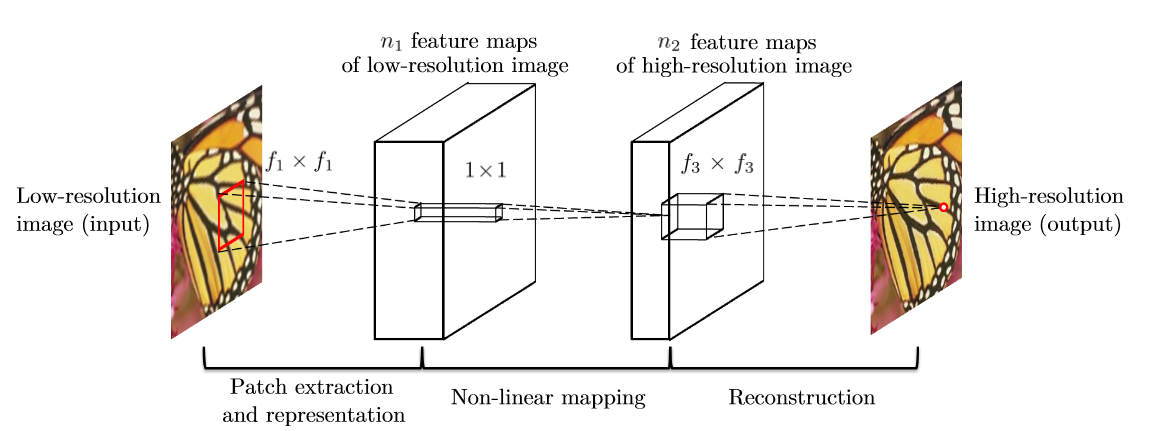
\includegraphics[width=1.0\textwidth]{imgs/SRCNN.png}
    \caption{SRCNN的结构}
    \label{fig:SRCNN}
\end{figure}

% \section{正则流模型}
% 正则流模型(Normalizing flow models)是一类基于可逆变换构建的概率生成模型,可用于生成复杂的高维数据分布。正则流模型包括了一系列从一个简单的先验分布(通常为高斯分布)开始,通过一系列可逆的变换(比如仿射变换,置换,仿射耦合层等)逐渐逼近目标分布的过程。这些可逆变换保证了模型的密度函数是可解的,并且可以直接计算概率密度函数和其对数的梯度。因此,正则流模型可以通过最大似然估计等优化方法来训练模型参数,实现对目标分布的拟合。我们假设随机变量$\mathbf{z}_0$经过$K$次参数为$\theta_i$可逆变换$f_i$生成数据$x$,则有
% \begin{equation}
%     \begin{aligned}
%         \mathbf{z}_0 &\sim p_0(z_0)\\
%         \mathbf{z}_i &= f_i(\mathbf{z}_{i-1}),i=1,2,3,\dots,K\\
%         x &= \mathbf{z}_K
%     \end{aligned}
% \end{equation}
% 为了确定$\theta_i$的值,可以使用极大似然估计:
% \begin{equation}
%     \log p(x)=\log p_0(z_0)-\sum_{i=1}^{K}\log|\det\frac{\text{d}f_i}{\text{d}z_{i-1}}|
% \end{equation}
% 此优化目标要求、

\section{超分辨率模型的评价指标}
为了能够评判各种超分辨率模型间精度的优劣,需要采用多种指标进行评价。而不同的评价指标则拥有不同的侧重点。
\subsection{基于参考的评价指标}
此类指标是最常用的评价指标。其中,PSNR(Peak Signal-to-Noise Ratio,峰值信噪比)通过比较原始图像与经过处理后的图像的信噪比来衡量两张图像之间的差距,单位为分贝(dB),取值范围为0到无穷大。PSNR越大,则说明两张图像越相近。PSNR的定义式为:
\begin{equation}
    \text{PSNR}=10\cdot \log_{10}(\frac{\text{MAX}_I^2}{\text{MSE}})
\end{equation}
其中,$MAX_I$是像素的最大值,这取决于像素值是$0\sim 255$还是$0\sim 1$;MSE(Mean Square Erros)是两张图像之间的均方误差。

SSIM\parencite{wang2002universal}(Structural Similarity Index Measure,结构相似性指标)除了考虑除了像PSNR考虑像素间差异以外,还考虑图像的结构、纹理、对比度等因素。SSIM没有单位,取值范围为-1到1,SSIM越大,说明两张图像相似度越高。SSIM的定义为
\begin{equation}
    \begin{aligned}
        SSIM(x,y)&=[l(x,y)s(x,y)c(x,y)]
                 &=\frac{(2\mu_x\mu_y+c_1)(2\sigma_{xy}+c_2)}{(\mu_x^2\mu_y^2+c_1)(\sigma_x^2+\sigma_y^2+c_2)}
    \end{aligned}
\end{equation}
其中,$l(x,y)$代表亮度,$s(x,y)$代表结构,$c(x,y)$代表对比度。$\mu_x$、$\mu_y$代表$x、y$的均值,$\sigma_x$、$\sigma_y$代表$x、y$的方差,$\sigma_{xy}$代表$x、y$的协方差,$c_1$、$c_2$为常数。实际计算中,采用滑动窗口法,即计算图像中每一个窗口的SSIM,最后取其平均值。

\subsection{基于感知的评价指标}
以上两种评价指标基本侧重于图像的像素和结构,二者的计算较为机械,有时候PSNR和SSIM指标高的图像并不能很好地满足人类的需求,故某些工作招募志愿者用肉眼对图像进行打分,但是这种评判方式具有较大的主观性,因此需要一个能够定量评判感知质量的评价指标。而LPIPS\parencite{zhang2018perceptual}(Learned Perceptual Image Patch Similarity,学习的图像像素相似性指标)就是其中具有代表性的一个指标。此指标通过卷积神经网络来学习人类对图像的感知差异。从计算方式上来说,此指标通过计算两张图像通过预训练的卷积神经网络提取得到的特征图之间的余弦距离来评判图像间的相似性,指标越接近于0,则说明两张图像在人类感知上越相近。由于侧重点不同,有时会出现LPIPS指标很优而PSNR/SSIM很劣或者PSNR/SSIM很优LPIPS很劣的情况,这个时候就要结合需求综合分析模型的优劣。